\begin{wrapfigure}{r}{0.45\textwidth}
  \vspace{-0.7cm}
  \begin{center}
    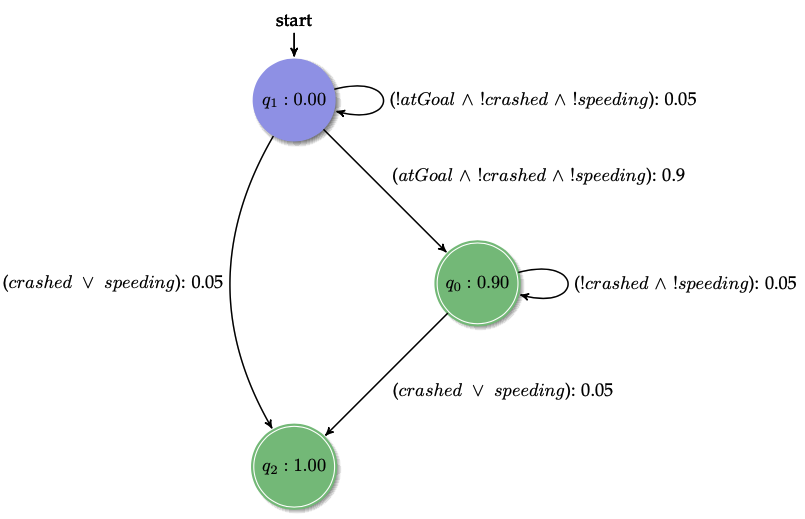
\includegraphics[width=0.45\textwidth]{Figures/PDFA.png}
  \end{center}
  \caption{An example of a probabilistic deterministic finite automaton (PDFA) specification for one of my toy autonomous driving scenarios.}
  \label{fig: driving_pdfa_spec}
\end{wrapfigure}

As an aerospace engineer, my interest in new, amazing machine learning technology like deep learning is somewhat tempered by the lack of explainability of Deep Neural Networks (DNNs), especially as pertaining to the solution of sequential decision-making problems. This means that while we have developed extensive methodologies in machine learning, \href{https://en.wikipedia.org/wiki/Motion_planning}{motion planning}, and \href{https://en.wikipedia.org/wiki/Formal_methods}{formal methods} for approaching humanity's desire for autonomous systems, but we currently lack robust ways to provide performance guarantees for autonomous, safety-critical systems. We are in dire need of more principled and guaranteed design methodologies than many "black-box" methods in use today if we want to realize trusted autonomy for safety-critical systems in our society.

\begin{wrapfigure}{l}{0.35\textwidth}
  \vspace{-0.7cm}
  \begin{center}
    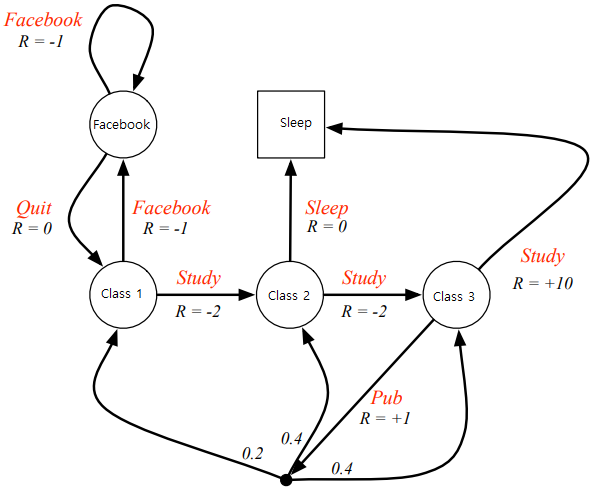
\includegraphics[width=0.35\textwidth]{Figures/MDP.png}
  \end{center}
  \caption{An example of a Markov Decision Process (MDP) for which we might want to learn a specification. (\href{https://medium.com/@bibekchaudhary/markov-decision-process-mdp-simplified-1ae44cf53cc1}{source})}
  \label{fig: mdp}
  \vspace{-0.3cm}
\end{wrapfigure}

To bring us closer to provably safe, interpretable decision-making algorithms for autonomous systems, one approach I am investigating is to use machine learning to learn high-level human goals from demonstrations in a format that is amenable to formal control synthesis. Autonomous vehicles exemplify an industry that currently faces many challenges in the field of decision making and control for a safety-critical system. In his annual review in 2018, Schwarting outlined the progress made in the Verification and Synthesis of decision-making and motion planning algorithms \cite{doi:10.1146/annurev-control-060117-105157}. Black box methods (i.e. DNN representing policy / value networks in Deep Reinforcement Learning) are struggling to be verified \cite{doi:10.1146/annurev-control-060117-105157}, which makes their use questionable in such a safety-critical environment. It was particularly noted that while formal control synthesis was of great interest, it does not see wide-spread use cause due to its expensive and the due to the difficulty in formally specifying desired system behavior.

My research consists of first using probabilistic state-machine learning algorithms (e.g. ALERGIA, MDI \cite{prob_state_merging_book}, or RTI(+) \cite{Verwer_PAutomaC}) to learn an automaton model for human demonstrator's specification for the operation of an autonomous system based on observed symbol sequences (traces) representing of system behavior. See Fig. \ref{fig: driving_pdfa_spec} for an example of such a specification. These probabilistic state machines allow are generative in nature, and when sampled from produce traces in the language of the probabilistic automaton. Then, using tools from formal methods, we compose this specification with a model for the autonomous system's dynamics (e.g. \href{https://en.wikipedia.org/wiki/Transition_system}{transition system} or \href{https://en.wikipedia.org/wiki/Markov_decision_process}{(PO)MDP} -- see Fig. \ref{fig: mdp}) to obtain a correct-by-construction policy to control the system model to follow the learned specification.

For this project, I would like to focus on the \textbf{specification learning} aspect of the project. While the methods mentioned earlier (ALERGIA, MDI, RTI(+)) work with a classical state-merging to merge the observed traces from the system's operation into a statistically consistent probabilistic state machine, I would like to investigate new works that leverage the amazing power of neural networks as probabilistic sequence models. This means that instead of directly learning a state machine from the observed traces, \textbf{I would like to experiment with using a learned DNN (probably a recurrent or attention model) to represent the language distribution over the given symbol alphabet, and then extract the language distribution from the DNN as a state machine.}

This sort of process is of interest to researchers working on explainable AI (XAI) as well as researchers like me working on formal control synthesis for uncertain sequential decision-making systems.